
\chapter{Background}
\label{chap:background}

This chapter explains the \textbf{basic concepts} used throughout the thesis. First, we explain \textbf{neural \acp{lm}}: from the basics of neural networks (§\ref{sec:nns}) and language modeling (§\ref{sec:lm-basics}), up to pretrained (§\ref{sec:plms}) and large language models (§\ref{sec:llms}). Then we move on to \textbf{\ac{d2t} generation}: covering rule-based (§\ref{sec:rule-d2t}) and neural-based systems (§\ref{sec:neural-d2t}), \ac{d2t} datasets (§\ref{sec:datasets}) and evaluation methods (§\ref{sec:evaluation}). We assume that the reader has certain expertise in related areas of \ac{nlp}, although not necessarily in \ac{nlg}. We aim to make the work self-contained by covering all the important concepts, pointing the interested reader to related work for more details.

Besides that, the chapter serves also as an \textbf{overview of the state of the art} in the fields of interest. In particular, the later subsections (\Cref{sec:plms,sec:llms} for neural \acp{lm} and \Cref{sec:neural-d2t,sec:datasets,sec:evaluation} for \ac{d2t} generation) describe the datasets, models, and metrics used for the experiments. As such, the chapter serves as the main point of reference; we will only briefly revisit the most relevant concepts in the respective chapters.


\section{Neural Language Models}
\label{sec:lms}
In this section, we work our way towards neural \acp{lm}: the mathematical foundations of \acp{nn} on which the neural \acp{lm} are built on (\autoref{sec:nns}), the basic ideas of language modeling (\autoref{sec:lm-basics}) and the way \acp{lm} are constructed, trained, and eventually applied in \ac{nlp} (\Cref{sec:plms,sec:llms}).

\subsection{Neural Networks}
\label{sec:nns}
First, we need to build a tool for learning patterns from data\footnote{Until we get to \ac{d2t} generation in \autoref{sec:d2t}, we will use the word ``\textit{data}'' only in its abstract sense, as in ``any inputs we can apply our algorithms to''. We will use the term ``structured data'' whenever it is necessary to make the distinction.}. This tool---which for us will be the \textbf{neural networks}---will later help us with learning patterns about language from large-scale textual data, and in turn with generating text.

Let's say our goal is to predict real-number output $y \in \mathbb{R}$ for the given vector of real numbers $\mathbf{x} = (x_1, \ldots, x_d) \in \mathbb{R}^d$.
% \footnote{We will follow the convention that vectors are denoted with boldface letters ($\mathbf{x}$), and real numbers with plain letters ($x$).} 
We assume that the $\mathbf{x} \rightarrow y$ mapping is not arbitrary (that would leave us with memorizing all the $(\mathbf{x},y)$ pairs), but follows some regularities and underlying patterns that can be learned. This assumption will be naturally satisfied if we consider $(\mathbf{x},y)$ to be representations of real-word data, e.g., documents and their labels.

For learning the underlying pattern between $\mathbf{x}$ and $y$, we will use mathematical models designed to capture the pattern in their parameters. The model estimates the parameters from a limited set of examples called the \textit{training data} and uses the learned parameters to predict the outputs on the \textit{test data}.

\paragraph{Perceptron Algorithm} One of the early mathematical models designed for predicting the outputs based on the inputs is the \emph{perceptron algorithm} (\citealp{rosenblatt1958perceptron}, \citealp[p.~192]{bishop2006pattern}). In this case, we assume the output is a binary class label: $y \in \{-1, 1\}$. The algorithm learns the parameters $\textbf{w} = (w_1, \ldots, w_d) \in \mathbb{R}^d$ and the bias $b \in \mathbb{R}$ describing a linear decision boundary separating the data points according to their class label. The algorithm proceeds as follows:


\begin{enumerate}
    \item The parameters $\textbf{w}$ and $b$ are initialized to small random values or zeros.
    \item For each training example $(\mathbf{x}_i, y_i)$, the algorithm updates the weights and bias to adjust their current estimate towards the ground truth target:
          \begin{align} \label{eq:perceptron1}
              \hat{y}_i  & = \text{sign}(\textbf{w} \cdot \mathbf{x} + b) \\
              \textbf{w} & = \textbf{w} + (y - \hat{y}) \textbf{x}        \\
              b          & = b + y - \hat{y}
          \end{align}
    \item The step (2) is repeated until convergence.
\end{enumerate}

The perceptron algorithm is guaranteed to converge if there exists a hyperplane which separates the data belonging to one class from another, otherwise it will not converge \cite{novikoff1962convergence}.

\paragraph{Multi-layer Perceptron} To overcome the fact that the perceptron is limited to linear decision boundaries, we can use a \textbf{\acl{mlp} (\acs{mlp}\glsunset{mlp}}; \citealp[p.~164]{goodfellow2016deep}). This mathematical model---also known as a feed-forward neural network---is able to approximate any bounded continuous function \cite{hornik1989multilayer}.

As the name suggests, \ac{mlp} uses multiple perceptron-like units called \textit{neurons}. Analogically to the perceptron (\autoref{eq:perceptron1}), each neuron computes its output $o$ using the rule:
\begin{align}
    o & = f(\mathbf{x}^\top \mathbf{w}  + b),
\end{align}
% \begin{itemize}
where $f: \mathbb{R} \rightarrow \mathbb{R}$ is the \emph{activation function}. Instead of signum, \ac{mlp} uses differentiable non-linear functions, most commonly nowadays \acl{relu} (\acs{relu}\glsunset{relu}; \citealp{nair2010rectified}) or its adapted version \acl{gelu} (\acs{gelu}\glsunset{gelu}; \citealp{hendrycks2016gaussian}).

For efficiency, the neurons are organized in layers, which enables formulating the \ac{mlp} computations in terms of matrix multiplication. The $i$-th layer of \ac{mlp} is parametrized with a matrix $\mathbf{W}_i \in \mathbb{R}^{d\times n}$ and a vector of biases $\mathbf{b}_i \in \mathbb{R}^{n}$, processing the \textit{hidden state} $\mathbf{h}_{i-1} \in \mathbb{R}^{d}$ (where we set $\textbf{h}_0 = \textbf{x}$):
\begin{align}
    \mathbf{h}_i & = f(\mathbf{h}_{i-1} \mathbf{W}_i + \mathbf{b}_i).
\end{align}
During training, we aim to minimize the \textit{loss function} describing the gap between the model predictions and the ground truth output. Since all the computations in \ac{mlp} are differentiable, we can use the chain rule to compute how each parameter in the network contributes to the loss. To minimize the loss, we use the \emph{backpropagation} algorithm \cite{kelley1960gradient,rumelhart1986learning}, updating the network parameters in the reverse order of layers. The magnitude of the updates is controlled by the learning rate parameter $\alpha$.

\paragraph{Recurrent Neural Networks} Unlike \acp{mlp}, where the size of the input is fixed, \acp{rnn} allow us to process a sequence of inputs $\mathbf{X} = (\mathbf{x}_1, \ldots, \mathbf{x}_n)$ of arbitrary length. Generally, an \ac{rnn} computes a sequence of hidden states $\mathbf{H} = (\mathbf{h}^{(0)}, \ldots, \mathbf{h}^{(n)})$ by repeatedly applying a function $f$ parametrized by the parameters of the network $\boldsymbol{\theta}$, the current input $\mathbf{x}_i$, and the previous hidden state $\mathbf{h}^{(i-1)}$ \cite[p.~367]{goodfellow2016deep}:
\begin{align}
    \mathbf{h}^{(i)} = f(\boldsymbol{\theta}, \mathbf{h}^{(i-1)}, \mathbf{x}_i).
\end{align}
The hidden state $\mathbf{h}^{(0)} \in \mathbb{R}^k$ is initialized randomly. After the input is processed, $\mathbf{H}$ contains an encoded representation of the sequence. The exact implementation of the function $f$ may vary, but is generally implemented as a series of matrix multiplications and non-linear functions.

Although \acp{rnn} are suitable for text processing and turned out to be have various successes in \ac{nlp} applications \TODO{cite}, they also have various shortcomings, including the limited dimensionality of the hidden state and limited possibilities of parallelization. However, they will serve as a stepping stone towards the transformer architecture described in \autoref{sec:lm-basics}.


\subsection{Text Representation}
\label{sec:lm-basics}
We will now look into the basics of text representation in neural networks.


\paragraph{One-Hot Encoding}
% Until now, we have assumed that the input to a network is a vector of real numbers. However, a
A text is a sequence of discrete units such as characters, words, or subwords. To convert these units---called \textit{tokens}---to a numerical representation, we can define a \textit{vocabulary} $V$ which assigns an integer index $i \in \{0, \ldots, |V|-1\}$ to each token.

The naive way to represent each token would be using its integer value. However, this would misleadingly suggest linear dependence between tokens. A better way is to use the index $i$ for constructing a \textit{one-hot} vector $\mathbf{x} \in \{0,1\}^{|V|} $ for each token:
\begin{align}
    x_j = \begin{cases}
        1 & \text{if } i = j, \\
        0 & \text{otherwise}.
    \end{cases}
\end{align}

While this representation is sound, it is quite sparse and does not capture the semantics of individual tokens, which puts high requirements on the representional capacity of the network.

\paragraph{Word Embeddings} To get a more useful representation of tokens, we may require that tokens with similar meaning are also close in the vector space. Using the distributional theory of meaning \cite{harris1954distributional,firth1957synopsis}, we can use the idea that tokens with similar roles also tend to occur in a similar context.

This idea is used in the Word2Vec algorithm \cite{mikolov2013distributed}. The algorithm extracts the token representations as the weights of an \ac{mlp} trained either for predicting the tokens in the neighborhood of each token (the \emph{skip-gram} objective) or vice versa, the token itself based on the tokens in its neighborhood (the \emph{continuous bag-of-words} objective). The output of the algorithm is an \textit{embedding matrix} $\mathbf{W}_e \in \mathbb{R}^{|V|\times d}$, which assigns each token a $d$-dimensional \textit{embedding vector} $\mathbf{x} \in \mathbb{R}^{d}$. The objectives are illustrated in \autoref{fig:word2vec}.

The idea of representing tokens with embedding vectors is employed in neural \acp{lm} described later in this section, even though the embedding matrix is not trained with the aforementioned algorithm, but joinly with the rest of the network.

\begin{figure*}[ht]
    \centering

    \begin{subfigure}{\textwidth}
        \centering
        \begin{subfigure}{0.45\textwidth}
            \centering
            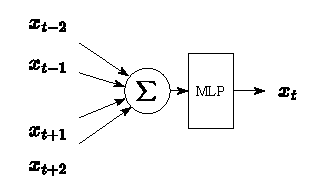
\includegraphics[width=\textwidth]{img/skipgram.pdf}
            \caption{Skip-gram}
            \label{fig:skipgram}
        \end{subfigure}
        \hspace{-20px}
        \begin{subfigure}{0.45\textwidth}
            \centering
            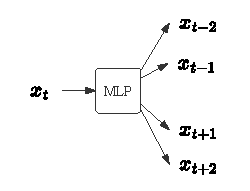
\includegraphics[width=0.75\textwidth]{img/cbow.pdf}
            \caption{Continuous Bag-of-Words}
            \label{fig:cbow}
        \end{subfigure}
    \end{subfigure}
    \caption{The objectives employed by the Word2Vec algorithm \cite{mikolov2013distributed}. In this case, the algorithm uses a context window of size $k=5$. In the (a) \emph{skip-gram} algorithm, we sum the embeddings of $k-1$ surrounding tokens and predict the original token. In the (b) \emph{continuous bag-of-words} algorithm, we use the original token for predicting the $k-1$ surrounding tokens.}
    \label{fig:word2vec}
\end{figure*}



\paragraph{Tokenization} We have also implicitly assumed that we have a way of splitting the text into tokens. Naively, we could split the text into words or characters. However, these approaches have their own shortcomings: word-level tokenization will not allow us to cluster together morphologically similar words, while character-level tokenization is computationally inefficient.

\emph{Subword tokenization}  is the middle ground between the two. The goal is to split the text into smaller pieces called \emph{subwords}, so that frequently used words will get their own subword, while less frequent words will be split into multiple subwords.

The subword tokenization algorithm that is frequently used in neural \acp{lm} is \emph{\ac{bpe}} \cite{sennrich2016neural}. The \ac{bpe} algorithm starts with the vocabulary of individual bytes, iteratively merging the most frequent tokens and adding them to the vocabulary $V$ until we reach the target vocabulary size. For example, the expression ``Subword tokenization'' could be split into four subwords \texttt{ ['Sub', 'word', '▁token', 'ization']}. The ``\texttt{▁}'' is a special character denoting a preceding space.


\subsection{Language Modeling}
Having a way to represent text, we can move on to processing it. Here, we will explain the notion of \emph{language modeling}.

\paragraph{Language Models} A useful formalism for text processing is a \emph{language model}: a mathematical model that estimates a probability of a sequence of tokens $S = (s_1, \ldots, s_n)$. For estimating the probability, we can factorize it into a product of conditional probabilities for each token using the chain rule:
\begin{align}
    P(S) = \prod_{i=1}^n P(s_i|s_1, \hdots, s_{i-1}).
\end{align}
Estimating the probability of longer sequences according to this formula is infeasible, as the model would require too many parameters. An \emph{\emph{n}-gram \ac{lm}} (parametrized by an integer \emph{N}) simplifies the product using the assumption that the probability of a token depends only on $N-1$ previous tokens:
\begin{align}
    P(S) = \prod_{i=1}^T P(s_i|s_{i-N+1}, \hdots,s_{i-1}).
\end{align}
The \emph{n}-gram \acp{lm} can be trained by estimating probabilities for individual \emph{n}-grams by tabulating their occurences in a text corpus. However, because of the limit on the length of the context for each token, the \emph{n}-gram \acp{lm} fail to capture long-term dependencies in the text.




\paragraph{Neural Language Model} A neural \ac{lm} is a \acl{lm} that estimates the text probability using a neural network. Denoting the parameters of the network by $\theta$ and the sequence of embeddings corresponding to $S$ as $\mathbf{X} \in \mathbb{R}^{|V|\times n}$:
\begin{align}
    P(S) = P_\theta(\mathbf{X}).
\end{align}
In contrast with \emph{n}-gram \acp{lm}, neural \acp{lm} can process the whole text, efficiently storing the probability estimates in its parameters, which makes it suitable for capturing long-term dependencies.

\subsection{Transformer Architecture}

Here, we will pave our way towards the transformer architecture, which is a core neural architecture used for \ac{nlp} nowadays.

\paragraph{Encoder-Decoder Framework}
We have described an \ac{rnn} (\autoref{sec:nns}) as a neural network that can process the sequence and \emph{encode} its representation in a sequence of hidden states. The idea behind the \emph{encoder-decoder framework} \cite{sutskever2014sequence,cho2014learning} is that we can \emph{decode} an output sequence with another network using the last hidden state of the encoder as its initial state. With \acp{rnn}, the workflow is the following:

\begin{enumerate}
    \item The \textbf{encoder} encodes the sentence of input embeddings $\mathbf{X}= (\mathbf{x}_1, \ldots, \mathbf{x}_n)$ into a hidden state $\mathbf{h}_e$ by repeatedly applying a transformation $\mathcal{E}$ in each timestep $t\in(1,n)$:
          \begin{align}
              \mathbf{h}_e^{(i)} = \mathcal{E}(\mathbf{h}_e^{(i-1)}, \mathbf{x}_i).
          \end{align}
    \item The \textbf{decoder} uses $\mathbf{h}_e^{(n)}$ as its initial state $\mathbf{h}_d^{(0)}$ and produces the sequence of output tokens  $Y = (y_1, \ldots, y_m)$ by repeatedly applying a transformation $\mathcal{D}$ in each timestep $j\in(1,m)$:
          \begin{align}
              \mathbf{h}_d^{(j)}, y_j = \mathcal{D}(\mathbf{h}_d^{(j-1)}, y_{j-1}).
          \end{align}
\end{enumerate}

\paragraph{Attention Mechanism} We have already mentioned that the hidden state of an \ac{rnn} has a fixed size, which limits the amount of information the network can capture about a sequence. The \emph{attention mechanism} \cite{bahdanau2015neural} as used in \acp{rnn} enables the decoder to extract the information dynamically from the encoded sequence. In each step $j$, the decoder computes a context vector $c_j$ as the weighted sum of the hidden states of the encoder $\{\mathbf{h}_e^{(0)}, \ldots, \mathbf{h}_e^{(n)}\}$ using the attention matrix $\mathbf{W}_a$:
\begin{align}
    \alpha_{ji}  & = \operatorname{softmax}(\mathbf{h}_d^{(j)}\mathbf{W}_a \mathbf{h}_e^{(i)}), \\
    \mathbf{c}_j & = \sum_i \alpha_{ji} \mathbf{h}_e^{(i)}.
\end{align}
The context vector is used as an additional input for the decoder:
\begin{align}
    \mathbf{h}_d^{(j)}, y_j = \mathcal{D}(\mathbf{h}_d^{(j-1)}, y_{j-1}, \mathbf{c}_j).
\end{align}


\paragraph{Self-attention Mechanism} Self-attention \cite{cheng2016long,vaswani2017attention} is a variant of the attention mechanism in which the source and the target sequence is identical. For the input $\mathbf{X} \in \mathbb{R}^{n,d}$, the \emph{self-attention} produces the output $\mathbf{H} \in \mathbb{R}^{n,d}$ of the same size. For each token, the resulting vector $\mathbf{h}_i \in \mathbf{H}$ is a weighed combination of the value vectors corresponding to all the tokens in a sequence (including the token itself):
\begin{align}
    \mathbf{h}_j = \sum_{i\in 1..n} \alpha_{ji} \mathbf{v}_i,
\end{align}
where the \emph{value vector} of each token is computed using a trainable \emph{value matrix} $\mathbf{W_v} \in \mathbb{R}^{n,d}$:
\begin{align}
    \mathbf{v}_i = \mathbf{x}_i \mathbf{W_v}.
\end{align}
To get the attention weights $\alpha_{ij}$, we first compute \textit{query} and \textit{key} vectors for each token using trainable matrices $\mathbf{W_q}$ and $\mathbf{W_k} \in \mathbb{R}^{n,d}$. Each weight is then a normalized dot product of the corresponding vectors:
\begin{align}
    \mathbf{q}_i & = \mathbf{x}_i \mathbf{W_q}                                                      \\
    \mathbf{k}_i & = \mathbf{x}_i \mathbf{W_k}                                                      \\
    \alpha_{ij}  & = \operatorname{softmax}\biggl(\frac{\mathbf{q}_i\mathbf{k}_j}{\sqrt{d}}\biggr).
\end{align}
The operations can be efficiently paralellized using matrix multiplication:
\begin{align}
    \mathbf{Q}                                             = \mathbf{X}\mathbf{W_q},\quad\mathbf{K} & = \mathbf{X}\mathbf{W_k},\quad\mathbf{V} = \mathbf{X}\mathbf{W_v}                           \\
    \operatorname{Attn}(\mathbf{Q}, \mathbf{K}, \mathbf{V})                                         & = \operatorname{softmax}\biggl(\frac{\mathbf{Q}\mathbf{K}^\top}{\sqrt{d}}\biggr)\mathbf{V}.
\end{align}


\paragraph{Transformer Architecture} The \emph{transformer}\footnote{Although \citet{vaswani2017attention} uses ``Transformer'' with a capital ``T'', the orthography is gradually shifting towards the variant with a lower-case ``t''. See, e.g., \citet[p.~215]{jurafsky2024}.} \cite{vaswani2017attention} is a neural network architecture which can process sequences efficiently in parallel. To achieve that, the transformer replaces the \ac{rnn} hidden state (which previously served for sharing information among tokens in a single sequence) with the self-attention mechanism applied over a series of layers.

Specifically, each layer is composed of two sublayers: (a) the \emph{self-attention layer} and (b) the \emph{\ac{mlp} layer}. The output of the $i$-th sublayer is added to its original input $\mathbf{H}^{(i)}$ in a so-called residual connection:
\begin{align}
    \mathbf{H}^{(i+1)} = \mathbf{H}^{(i)} + \operatorname{sublayer}(\mathbf{H}^{(i)}).
\end{align}
The sublayers serve a different purpose: while the \ac{mlp} layer computes element-wise operations over each token, the self-attention layer enables sharing information among tokens. The sublayer input (or output, depending on the architecture variant) is normalized using \emph{layer normalization} \cite{ba2016layer}.

To get the input representation $\mathbf{H}^{(0)}$, we sum the token embeddings $\mathbf{X} \in \mathbb{R}^{n,d}$ with \emph{positional embeddings}. Positional embeddings encode the information about the absolute or relative position of individual tokens which would otherwise get lost in parallelized processing. See \citet{dufter2022position} for an overview of positional embedding variants.


\begin{figure*}[ht]
    \centering
    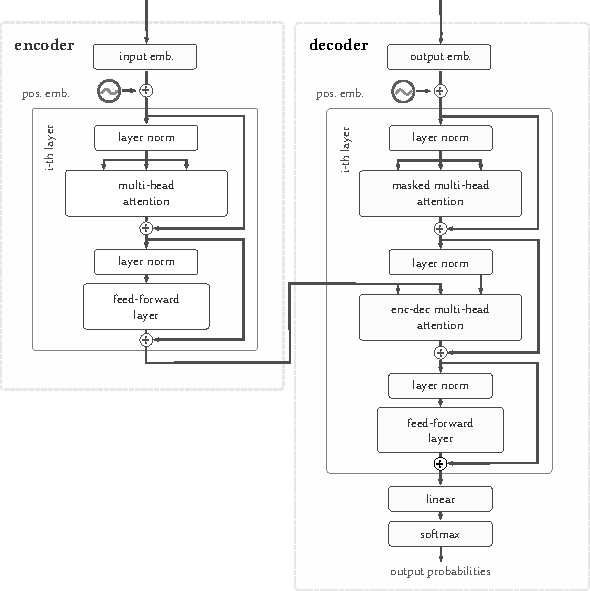
\includegraphics[width=0.9\textwidth]{img/transformer.pdf}
    \caption{An encoder-decoder variant of the Transformer architecture. The encoder has $N_{e}$ layers, each consisting of a self-attention and MLP sublayer. The decoder has $N_{d}$ layers with masked self-attention and encoder-decoder attention, again followed by an MLP sublayer. The input to each sublayer is normalized using layer norm. After the last decoder layer, the output probabilities are computed using a linear projection and softmax. The figure is adapted from \href{https://github.com/bbycroft/llm-viz/blob/main/src/llm/intro-image.svg}{https://github.com/bbycroft/llm-viz}.}
    \label{fig:transformer}
\end{figure*}


For each token in the sequence, we train the model to maximize the log probability (i.e., minimize the negative log probability) of the ground truth token $y_i$ given the previous sequence of tokens in the sequence:
\begin{align}
    \operatorname{loss}_i = -\log P_\theta(y_i|y_1, \hdots, y_{i-1}).
\end{align}
Training the transformer model is \emph{self-supervised}: each token in the training sequence serves as the ground-truth ``\emph{label}'' that the model aims to predict. We train the model on \emph{batches} of data, using an optimization algorithm such as \acl{sgd} (\acs{sgd}\glsunset{sgd}; \citealp[p.~275]{goodfellow2016deep}) or Adam \cite{kingma2014adam}. The batch size $b$ and the learning rate $\alpha$ are the training hyperparameters.

As shown in \autoref{fig:transformer}, the original Transformer architecture follows the encoder-decoder framework. The encoder layers follow an aforementioned scheme, while the decoder layers have the following differences:
\begin{itemize}
    \item Each layer contains another sublayer called the \emph{encoder-decoder attention}. In contrast to the self-attention mechanism, the \emph{keys} and \emph{values} come from the last layer of the encoder, enabling the decoder to attend to the encoded sequence.
    \item The self-attention is \emph{masked} so that each token can collect information only from the preceding tokens, which is necessary to enable text generation using left-to-right autoregressive decoding.
\end{itemize}
After the last decoder layer, the hidden states are projected into a matrix of size $\mathbb{R}^{|V|\times n}$ and normalized using softmax, producing a probability distribution over the vocabulary for each input token.

\paragraph{Text Generation} As we mentioned, we can use \textit{left-to-right autoregressive decoding} for generating text. The decoding process starts by feeding a special \texttt{<s>} (beginning of sequence) token into the decoder and then iteratively selecting the \emph{i}-th token based on the probability distribution for the \emph{i}-th position, until the  \texttt{</s>} (end of sequence) token is decoded. The procedure is outlined in Algorithm \ref{alg:decoding}.
\begin{algorithm}[ht]
    \begin{algorithmic}[1]
        \State{Initialize: $Y= \texttt{<s>}, t = \texttt{<s>}$ \Comment{Output sequence, current token}}
        \While{$t \neq \texttt{</s>}$}
        \State Predict next token probability distribution: $p(t | Y)$
        \State Sample next token: $t \sim p(t | Y)$ \label{alg:dec:sample}
        \State Update output sequence: $Y = Y \cup t$
        \EndWhile
        \State Return $Y$
    \end{algorithmic}
    \caption{Autoregressive decoding}
    \label{alg:decoding}
\end{algorithm}

\noindent The sampling step (line \ref{alg:dec:sample}) can be realized in various ways, including:
\begin{itemize}
    \item \textbf{Greedy decoding}: Select the most probable token.
    \item \textbf{Top-$k$ sampling}: Sample the next token from the $k$ most probable tokens.
    \item \textbf{Top-$p$ (nucleus) sampling} \cite{holtzman2019curious}: Sample the next token from the tokens with cumulative probability $p$.
    \item \textbf{Beam search}: Extend the $k$ most probable sequences from the previous step with the next tokens, keep the $k$ most probable sequences for the next step.
\end{itemize}
While the greedy decoding and beam search are used to decode more probable sentences, the sampling algorithms are used for decoding more creative outputs. The algorithms can be also combined together.

\subsection{Pretrained Language Models}
\label{sec:plms}
It turns out that training a transformer model from scratch is mostly not practical: it requires non-trivial computational resources, large-scale data sources, and extensive training time. The workflow that gradually established after the introduction of the transformer architecture is thus following: the models are first \emph{pretrained} using a generic objective on large-scale data, and then \emph{finetuned} for downstream tasks on a task-specific dataset.


\paragraph{Model types} Depending on the downstream task, different variants of the transformer architecture may be used (see \autoref{tab:pretrained_models} for an overview):

\begin{itemize}
    \item \textbf{Encoder models} -- The models use only the \emph{encoder} part of the transformer architecture. These models are trained using the \emph{\ac{mlm} objective}: predicting tokens on the masked positions in the sequence. The output of these models is a contextualized representation of the input sequence, which can be used for tasks such as sequence classification, sequence tagging, or computing sequence similarity.
    \item \textbf{Encoder-decoder models} -- The models use the original \emph{encoder-decoder} architecture. These models are usually trained using a variant of denoising objective: predicting the original sequence from its corrupted version. The models are mostly used for sequence-to-sequence tasks, such as machine translation, question answering or summarization.
    \item \textbf{Decoder models} -- The models use only the \emph{decoder} part of the transformer architecture. These models are trained using the \emph{causal language modeling objective}: predicting the next token in a sequence. The models are suitable for unconditional text generation, but they can also used for the same tasks as the encoder-decoder models, using the input sequence as the ``pre-generated'' output prefix.
\end{itemize}

\begin{table}[t]
    \footnotesize
    \centering
    \begin{tabular}{lp{4.5cm}ll}
        \toprule
        \textbf{Type}            & \textbf{Pretraining Objective}            & \textbf{Model}                                       & \textbf{\# Parameters} \\
        \midrule
        \multirow{2}{*}{Encoder} & \multirow{2}{*}{Masked Language Modeling} & BERT \cite{devlinBERTPretrainingDeep2019}            & 110M-340M              \\
                                 &                                           & RoBERTa \cite{liuRoBERTaRobustlyOptimized2019}       & 125M-355M              \\
                                 &                                           & \textsc{LaserTagger} \cite{malmi2019lasertagger}     &                        \\
        \midrule
        \multirow{2}{*}{Enc-Dec} & \multirow{2}{*}{Text Denoising}           & BART \cite{lewisBARTDenoisingSequencetoSequence2019} & 139M-406M              \\
                                 &                                           & mBART \cite{liuMultilingualDenoisingPretraining2020} & 880M                   \\
                                 &                                           & T5 \cite{raffelExploringLimitsTransfer2019}          & 220M-11B               \\
        \midrule
        Decoder                  & Causal Language Modeling                  & GPT-2 \cite{radfordLanguageModelsAre2019}            & 117M-1.5B              \\
                                 &                                           & Llama2 \cite{touvronLlamaOpenFoundation2023}         & 7B-70B                 \\
                                 &                                           & Mistral \cite{jiangMistral7B2023}                    & 7B-70B                 \\
                                 &                                           & Zephyr \cite{tunstallZephyrDirectDistillation2023}   & 7B-70B                 \\
        \bottomrule
    \end{tabular}
    \caption{Types of transformer architectures, along with specific models used in this work. The number of parameters may vary based on the model variant.}
    \label{tab:pretrained_models}
\end{table}

\paragraph{Finetuning} By \emph{finetuning} a model we mean additional training of a pretrained model on a task-specific dataset. Finetuning is more cost- and data-efficient than training a model from scratch, but is typically used only for a single task, since repeated model update can lead to erasing previous knowledge, also known as ``catastrophic forgetting'' \cite{mccloskey1989catastrophic,kirkpatrick2017overcoming}.


\paragraph{Few-shot and Zero-shot Settings} If the training data available to the model is very limited (no more than \textasciitilde 100 examples), we talk about a \emph{few-shot} setting. By taking it to the extreme, we arrive to a \emph{zero-shot} setting, in which we use a model on the task for which it has not been trained for. Making the models work in these settings is crucial for using the models in low-resource scenarios.

\subsection{Large Language Models}
\label{sec:llms}
Scaling the models in terms of the number of parameters and the size of the training data has turned out to further improve the performance of the models \cite{kaplan2020scaling,hoffmann2022training}. Larger models were shown to exhibit unprecedented capabilities in terms of language fluency, language understanding, and reasoning skills \cite{wei2022emergent,bubeck2023sparks}, giving name to a specific category of \emph{\aclp{llm} (\acsp{llm}\glsunset{llm};} \citealp{brown2020language,zhao2023survey}). \Acp{llm} are generally larger than 1B parameters and based on the transformer decoder architecture. For many \ac{nlp} tasks, \acp{llm} have comparable or better performance than previous task-specific approaches.

\paragraph{In-context Learning} The general knowledge of \acp{llm} can be leveraged for performing on novel tasks without the need for finetuning on task-specific data. Instead, the task can be formulated in a natural language prefix (commonly called a \emph{prompt}), and the model completes the task by causal language modeling. This ability is known as \emph{in-context learning} \cite{brown2020language,dong2022survey}. If the model is given a limited set of input-output examples in the prompt, we talk about \emph{few-shot prompting}; if the model is given no examples, we talk about \emph{zero-shot prompting}.

\paragraph{Instruction Tuning} The key to strong cross-task of \acp{llm} is instruction tuning: finetuning on a large dataset of tasks formulated using natural language instructions, such as \textit{``Answer this question: \{question\}''} or \textit{``Translate this sentence: \{sentence\}''} \cite{sanh2021multitask,ouyang2022training}. The instruction-tuned models can be then easily \emph{prompted} to perform a task of choice, even if   they were not directly trained for the task.



\section{Data-to-Text Generation}
\label{sec:d2t}
In this section, we will provide background for the task of \ac{d2t} generation. After presenting the basic set of \ac{d2t} tasks (\autoref{sec:d2t-tasks}), we will discuss the rule-based (\autoref{sec:rule-d2t}) and neural (\autoref{sec:neural-d2t}) \ac{d2t} generation systems, and describe the datasets used throughout this work (\autoref{sec:datasets}). Lastly, we will present the evaluation metrics used in \ac{d2t} generation (\autoref{sec:evaluation}).

\subsection{Applications}
\label{sec:d2t-tasks}

\ac{d2t} generation is a catch-all term for tasks which require \emph{mapping structured data to natural language}. The structured data can take various forms: tabular databases, graphs and knowledge bases, time-series, or charts \cite{gattSurveyStateArt2018,sharmaInnovationsNeuralDatatotext2022}. The form of the input structured data is usually the defining feature of the \emph{dataset} and the related \emph{modeling approaches} (cf. \autoref{sec:datasets}). Practical applications, on the other hand, may combine multiple data formats and approaches.

Here is a brief overview of applications of \ac{d2t} generation:

\begin{itemize}
    \item \textbf{Automated Journalism}: Augmenting (or in simple cases, even replacing) human journalists for writing data-based reports, including:
          \begin{itemize}
              \item \textbf{News reports}: Automating news writing in various domains, such as election results \cite{leppanen2017data}, incidents \cite{vanderleeCACAPODatasetMultilingual2020}, earthquakes \cite{oremus2014first}, or wildlife tracking \cite{siddharthan2012blogging,ponnamperuma2013tag2blog}.
              \item \textbf{Sport reports}: Generating game summaries for sports with rich data capturing the course of the game, such as basketball \cite{wiseman2017challenges,thomson2020sportsett}, baseball \cite{puduppullyDatatotextGenerationEntity2019} or soccer \cite{van2017pass}.
              \item \textbf{Financial reports}: Supporting financial decisions by generating comments on stock prices \cite{murakami2017learning,aoki2018generating} or summaries of financial documents \cite{chapman2022towards}.
              \item \textbf{Weather reports}: Generating weather forecasts and weather-related reports \cite{goldberg1994using,belz2005corpus,belz2008automatic,angeli-etal-2010-simple,balakrishnan2019constrained}.
          \end{itemize}
    \item \textbf{Business Intelligence Reports}: Providing decision support in business reports alongside data summaries and visualizations (mostly commercial companies such as \href{https://www.arria.com}{Arria}, \href{https://infosentience.com}{InfoSentience}, or \href{https://www.vphrase.com}{vPhrase}; see \citealp{daleNavigatingTextGeneration2023} for a recent overview),
    \item \textbf{Chart Captioning}: Generating captions\footnote{In contrast to image captioning \cite{stefanini2022show}, here the systems can rely on the underlying data in textual form (although the approaches can be hybrid, see e.g. \citealp{kantharaj2022chart}).} for charts or graphs, e.g., for assistive technologies (such as screen readers), document indexing, or simplifying decision support \cite{demirGeneratingTextualSummaries2008,demirSummarizingInformationGraphics2012,obeidCharttoTextGeneratingNatural2020,kantharaj2022chart}.
    \item \textbf{Healthcare Summaries}: Providing  clinical data summaries about patients to clinicians \cite{portet2009automatic,scott2013data}, or vice versa, providing information to patients for behavioral change \cite{reiter2003lessons} or nutritional counseling \cite{balloccu-reiter-2022-comparing}.
    \item \textbf{Product Descriptions}: Automating generating product descriptions in e-commerce, either domain-specific approaches for products such as laptops and TVs \cite{wen2015toward,wen2016multi}, or general-domain approaches for big e-commerce platforms \cite{shaoControllableDiverseText2021,kotoCanPretrainedLanguage2022}.
\end{itemize}

\subsection{D2T Generation Pipeline}
\label{sec:d2t-pipeline}
Until recently, these tasks could not be realized in end-to-end fashion. Typically, the systems decomposed the tasks into a pipeline of approximately 4-6 subtasks\footnote{Some tasks may be further subdivided, which can generate up to 10 subtasks as in \citet{milleModD2TMultilayerDataset2023}.}, starting with structured data and finishing with the text in natural language \cite{reiterBuildingAppliedNatural1997,reiterArchitectureDatatoTextSystems2007,gattSurveyStateArt2018}. Here we selected five representative subtasks illustrated in \TODO{figure}:

\begin{enumerate}
    \item \textbf{Content Determination}: Deciding which facts from the structured data
          to include in the text.
    \item \textbf{Document Planning}: Determining the order of the
          facts, dividing them into paragraphs.
    \item \textbf{Sentence Planning}: Aggregating the facts into
          sentences.
    \item \textbf{Lexicalisation}: Transforming the facts to text segments.
    \item \textbf{Surface Realisation}: Combining the text segments into a well-formed text in natural language.
\end{enumerate}

Decomposing \ac{d2t} generation into subproblems---where each module tackles a simple task---helps to modularize the system. Since each module has a specific and well-defined function, it makes the system as a whole more explainable. Modularization also enables realizing each part of the system using a different approach, from rule-based and grammar-based approaches up to neural models.

The subtasks are typically executed in a \emph{pipeline}, meaning the output from one module serves as the input to another. The pipeline-based approach can lead to error accumulation, propagating errors to downstream modules. Despite these issues, the pipeline approach remains a cornerstone approach for grammar-based surface realization systems such as FORGe \cite{milleFORGeWebNLG20172017,mille2019teaching} and it is employed in software frameworks such as SimpleNLG \cite{gatt2009simplenlg}. It also brings benefits to neural-based systems \cite{ferreiraNeuralDatatotextGeneration2019}, as we will explore in \autoref{sec:pipeline}.


\subsection{Pre-Neural Approaches}
\label{sec:rule-d2t}

By \emph{pre-neural approaches} for \ac{d2t} generation, we mean computational approaches for tackling the task which do not rely on neural models. We can generally divide them into rule-based approaches, grammar-based approaches, and data-driven approaches. These approaches were prevalent until cca 2018, when neural approaches started to gain traction, and are still in use in various forms until today \cite{gattSurveyStateArt2018,daleNaturalLanguageGeneration2020,daleNavigatingTextGeneration2023}.

\paragraph{Rule-based Approaches} Rule-based systems are often characterised by \emph{templates}: pre-written text snippets which are enriched with values from the data. Templates can range from simple fill-in-the-blank approaches (such as \textit{``The temperature will be \{temp\} degrees''}) to more sophisticated templates using a templating language \cite{reiter2016nlg,gatt2009simplenlg}.  Hand-written rules are used for not only selecting the templates, but also for filling the placeholders with values (which can be non-trivial in languages with rich morphology), and combining the templates together. The resulting rule-based system is usually tied to the specific task and domain and cannot handle more complex cases, but can be way to generate sufficient outputs with reasonable development time and costs \cite{vanderleeAutomatedLearningTemplates2018}.

Outside of lexicalization and surface realization, rule-based approaches can be also used in earlier stages of the \ac{d2t} generation pipeline (cf. \autoref{sec:d2t-pipeline}). In the content selection step, domain-specific heuristics can be used for extracting important information from the data, e.g., \textit{``if a spike is over a certain threshold, include it in the report''} \cite{portet2009automatic,gkatzia2016content}. In the text planing step, various schemata can be used for determining an appropriate discourse structure, e.g., \textit{``if a player
    scores two consecutive goals, describe these in the same sentence''} \cite{mckeown1985discourse,gattSurveyStateArt2018}.

\paragraph{Grammar-based Approaches}
\paragraph{Data-driven Approaches}



\subsection{Neural Approaches}
\label{sec:neural-d2t}
\subsection{Datasets}
\label{sec:datasets}
\subsection{Evaluation Metrics}
\label{sec:evaluation}